\documentclass[12pt]{article}
\title{ECE M16 Final}
\usepackage{subcaption}
\author{Lawrence Liu}
\usepackage{graphicx}
\usepackage[english,shorthands=off]{babel}        % shorhands=off is required for babel french in combination with tikz karnaugh....
\usepackage[utf8x]{inputenc}
\usepackage[T1]{fontenc}
\usepackage{amsmath}
\usepackage{geometry}
\geometry{verbose,a4paper, tmargin=3.5cm,bmargin=3.5cm,lmargin=2.5cm,rmargin=2.5cm,headsep=1cm,footskip=1.5cm}
\usepackage{colortbl}
\usepackage[dvipsnames]{xcolor}
\usepackage{tikz -timing}
\usepackage{tikz}
\usepackage{listings}
\usetikzlibrary{karnaugh}

\definecolor{LogisimKMapColor0}{RGB}{128,0,0}
\definecolor{LogisimKMapColor1}{RGB}{230,25,75}
\definecolor{LogisimKMapColor2}{RGB}{250,190,190}
\definecolor{LogisimKMapColor3}{RGB}{170,110,40}
\definecolor{LogisimKMapColor4}{RGB}{245,130,48}
\definecolor{LogisimKMapColor5}{RGB}{255,215,180}
\definecolor{LogisimKMapColor6}{RGB}{128,128,0}
\definecolor{LogisimKMapColor7}{RGB}{255,255,25}
\definecolor{LogisimKMapColor8}{RGB}{210,245,60}
\definecolor{LogisimKMapColor9}{RGB}{0,0,128}
\definecolor{LogisimKMapColor10}{RGB}{145,30,180}
\definecolor{LogisimKMapColor11}{RGB}{60,180,175}
\definecolor{LogisimKMapColor12}{RGB}{0,130,203}
\definecolor{LogisimKMapColor13}{RGB}{230,190,255}
\definecolor{LogisimKMapColor14}{RGB}{170,255,195}
\definecolor{LogisimKMapColor15}{RGB}{240,50,230}


\definecolor{codegreen}{rgb}{0,0.6,0}
\definecolor{codegray}{rgb}{0.5,0.5,0.5}
\definecolor{codepurple}{rgb}{0.58,0,0.82}
\definecolor{backcolour}{rgb}{0.95,0.95,0.92}

\lstdefinestyle{mystyle}{
    backgroundcolor=\color{backcolour},   
    commentstyle=\color{codegreen},
    keywordstyle=\color{magenta},
    numberstyle=\tiny\color{codegray},
    stringstyle=\color{codepurple},
    basicstyle=\ttfamily\footnotesize,
    breakatwhitespace=false,         
    breaklines=true,                 
    captionpos=b,                    
    keepspaces=true,                 
    numbers=left,                    
    numbersep=5pt,                  
    showspaces=false,                
    showstringspaces=false,
    showtabs=false,                  
    tabsize=2
}

\lstset{style=mystyle}

\begin{document}
\maketitle
\section*{Problem 1}
\begin{center}
\begin{tabular}{c| c c c c}
    & 1 & 1 & 0 & 1\\
    \cline{2-5}
    1 & 11 & 00 & 00 & 10 \\
    & 1 & & &\\
    \cline{2-2}
    101 & 10 & 00 & &\\
    & 1 & 01 & &\\
    \cline{2-3}
    1100 & & 11 & 00 &\\
    & & 0 & &\\
    \cline{3-4}
    & & 11 & 00 & 10\\
    11001 & & 1 & 10 & 01\\
    \cline{3-5}\\
    & & 1 & 10 & 01
    
\end{tabular}
\end{center}
\section*{Problem 2}
Basing on the assumption that $c[1:0]=11$ corresponds with $o[1:0]=i[1:0]$
we have that 
\begin{align*}
    a[1]&=\overline{c[1]}.\overline{c[0]}.i[7]+\overline{c[1]}.c[0].i[5]+
        c[1].\overline{c[0]}.i[3]+c[1].c[0].i[1]\\
        &=\overline{c[1]}.(\overline{c[0]}.i[7]+c[0].i[5])+c[1].(\overline{c[0]}.i[3]+c[0].i[1])
\end{align*}
\begin{align*}
    a[0]&=\overline{c[1]}.\overline{c[0]}.i[6]+\overline{c[1]}.c[0].i[4]+
        c[1].\overline{c[0]}.i[2]+c[1].c[0].i[0]\\
        &=\overline{c[1]}.(\overline{c[0]}.i[6]+c[0].i[4])+c[1].(\overline{c[0]}.i[2]+c[0].i[0])
\end{align*}
Which results in a circuit like this\\
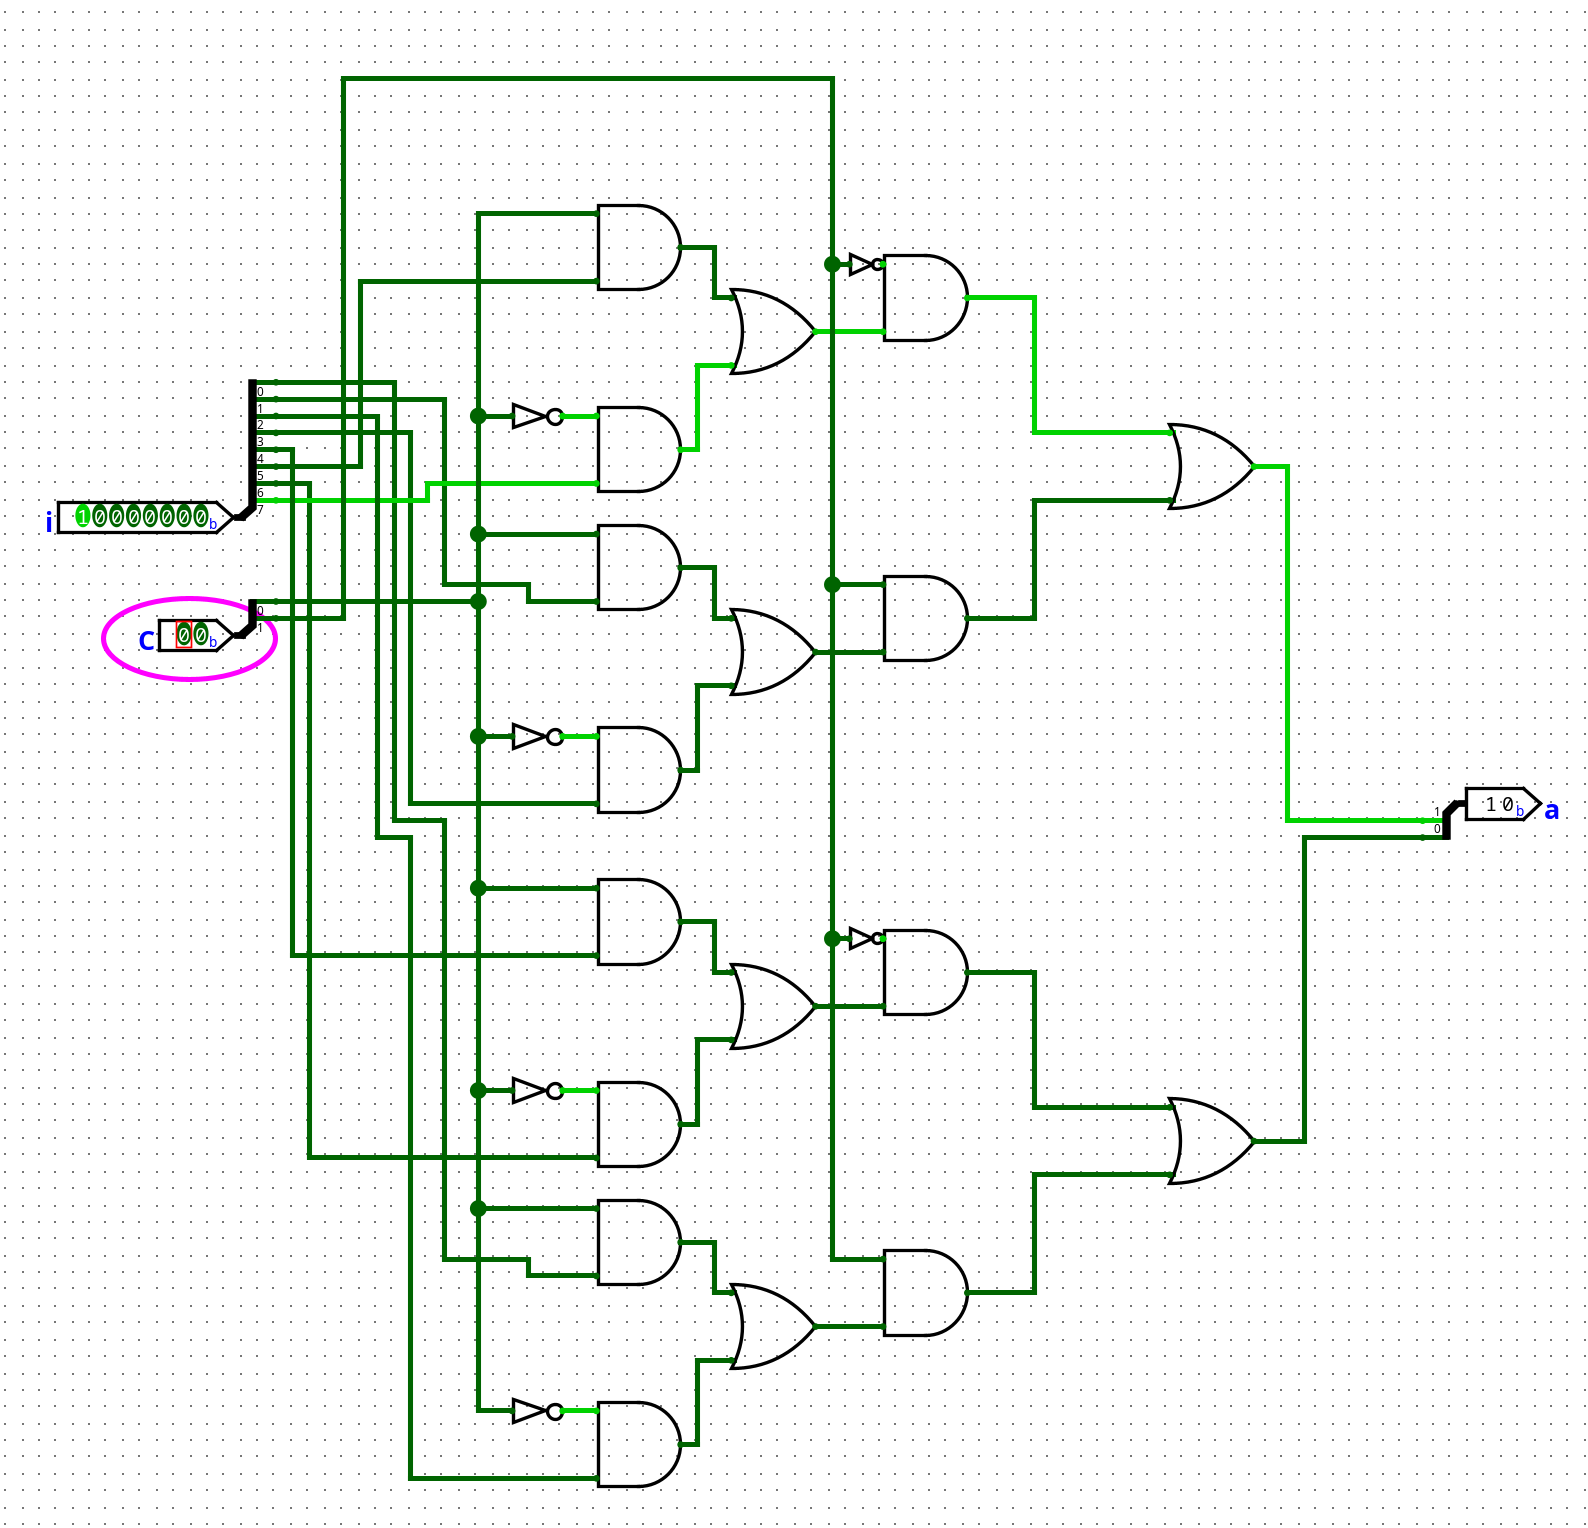
\includegraphics[scale=0.25]{fig1.png}
\section*{Problem 3}
I created the circuit, and it is shown above, and I tested it with the following python checker srcipt
\lstinputlisting[language=Python]{checker.py}
This script utilizes Logisim's command line ability. I had the files in the following format
\begin{verbatim}
ECEM16
 |- .gitignore
 |- Final
 | |-logisim
 | | |- FinalQ3.circ
 | :
 | :
 | |- checker.py
 |- .gitignore
 |- logisim-evolution.jar
\end{verbatim}
\section*{Problem 4}
Let $c[1:0]$ be the desired output from our counter: we want the following timing diagram:
\\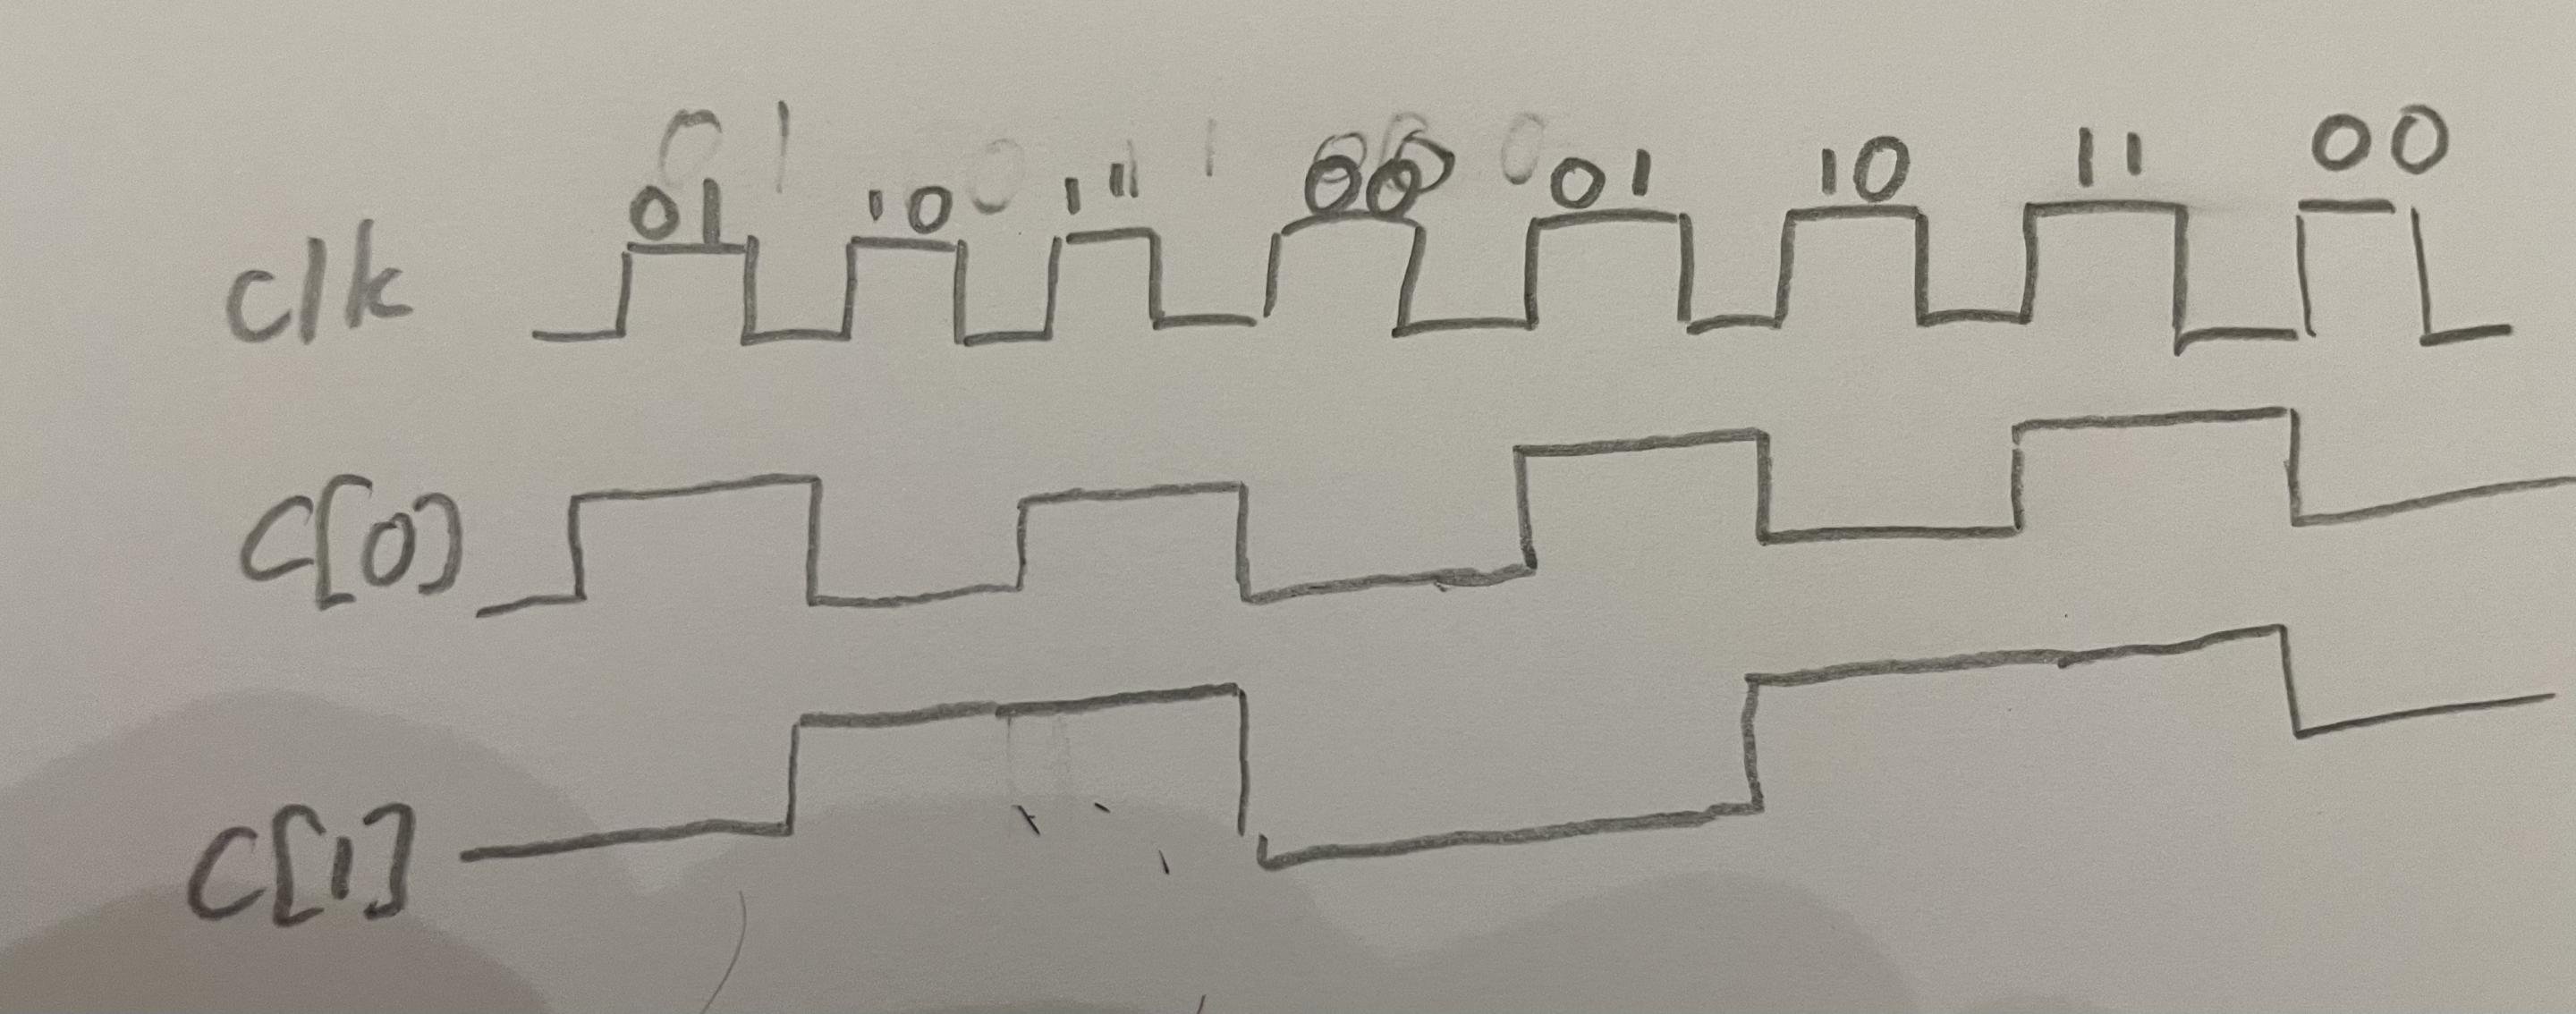
\includegraphics[scale=0.15]{fig4.jpg}\\
The first thing we notice is that $c[0]$ is just the clock input 
but with a period twice of clock, and $c[1]$ is just the clock input 
with a period of 4 times clock. We can make the output from a circuit 
toggle with each clock pulse (ie doubling its frequency), by connecting
$\overline{Q}$ with $D$, in the following manner:\\
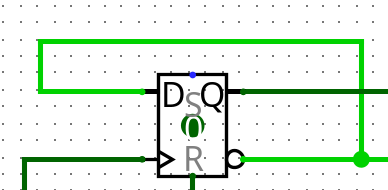
\includegraphics[scale=0.5]{fig5.png}\\
Likewise we can make the output from a circuit toggle with every other clock pulse 
(thereby multiplying its period by 4) by connecting two flip flops in the following manner\\
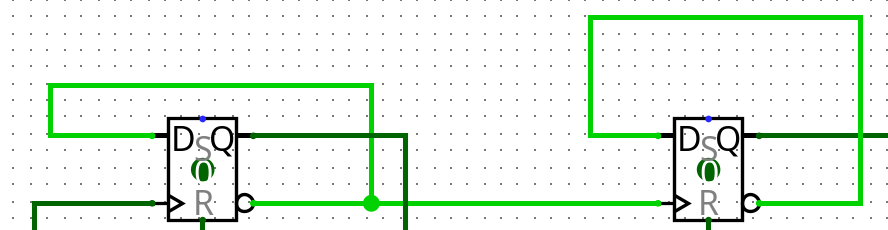
\includegraphics[scale=0.5]{fig6.png}\\
Therefore we have the following circuit:\\
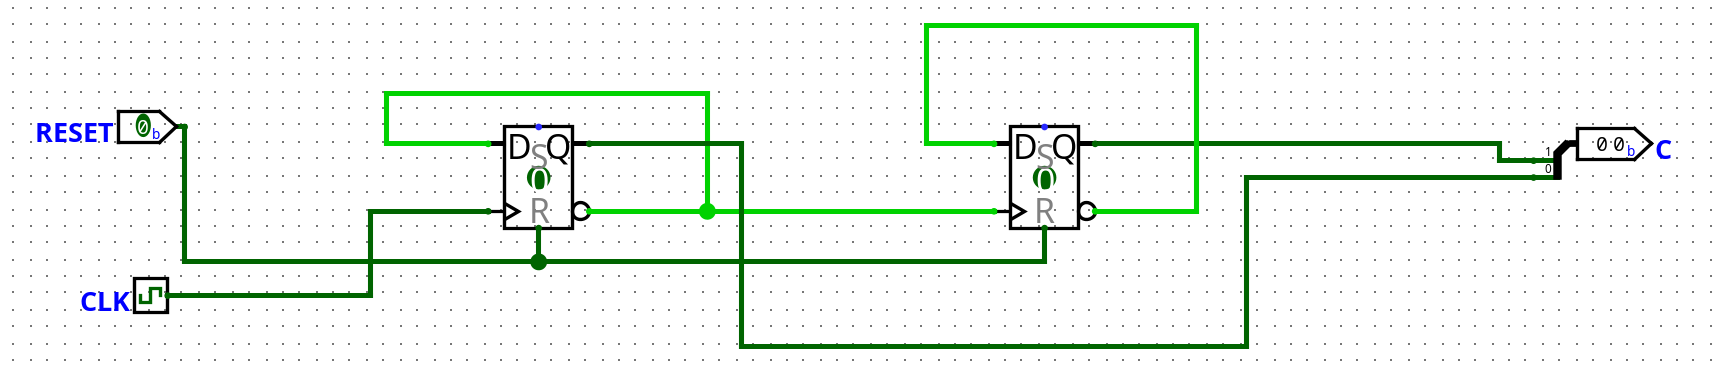
\includegraphics[scale=0.25]{fig7.png}
\section*{Problem 5}
I created the circuit, and it is shown above, and I tested 
by comparing its output vs that of a logisim counter, its output is denoted
as test in the chronograph below.\\
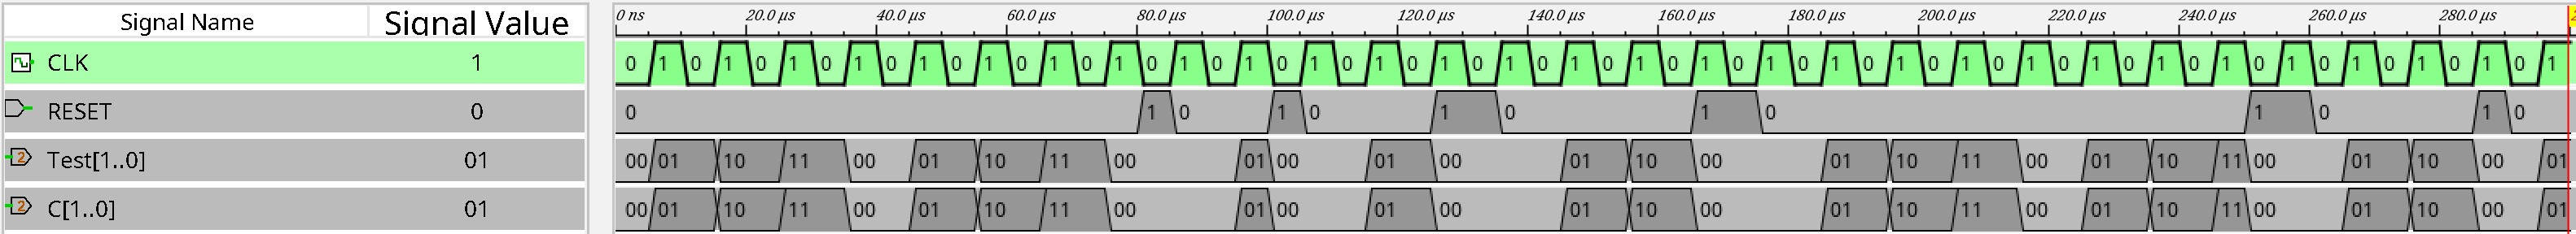
\includegraphics[scale=0.2]{fig8.png}
As one can see, the chronograph outputs of my counter vs logisim's counter is the same.
\section*{Problem 6}

We have the following transition table:
\begin{center}
    \begin{tabular}{|c|c|c|c|c|c|c|c|}
    & Prev state& \multicolumn{4}{c}{Inputs (REQ,DONE)} & \multicolumn{2}{c}{OUTPUT} \\
    \hline
    & $(y_1y_0)^n$ &0,0 &0,1 &1,1 &1,0 & GO & ACK\\
    \hline
    S1 & 0,0 & S1 & & &S2 & 0 & 0\\
    \hline
    S2 & 0,1 & & &S3 &S2 & 1 & 0\\
    \hline
    S3 & 1,1 &S4 & & &S3 & 0 & 1\\
    \hline
    S4 & 1,0 &S4 & S1& & &1 & 1\\       
    \end{tabular}

\end{center}
The corresponding state diagram is shown below.\\
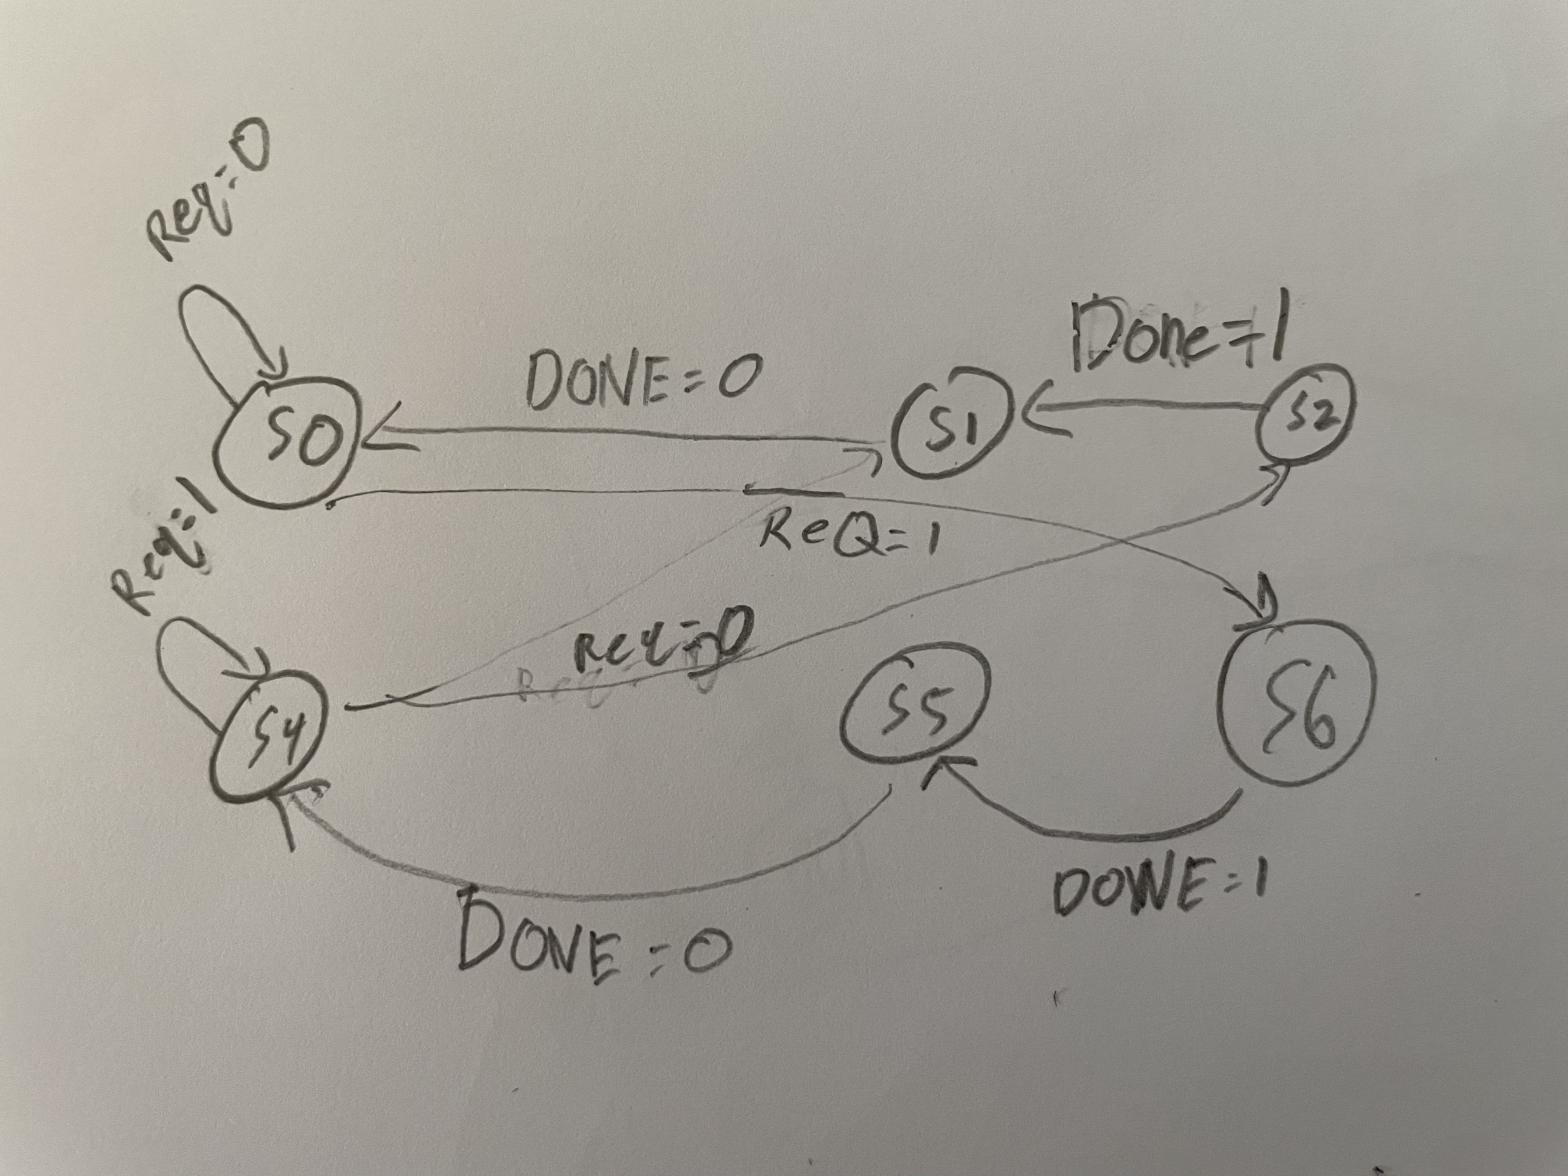
\includegraphics[scale=.075]{fig11.jpg}

And it results in the following kmap for $y_1$\\
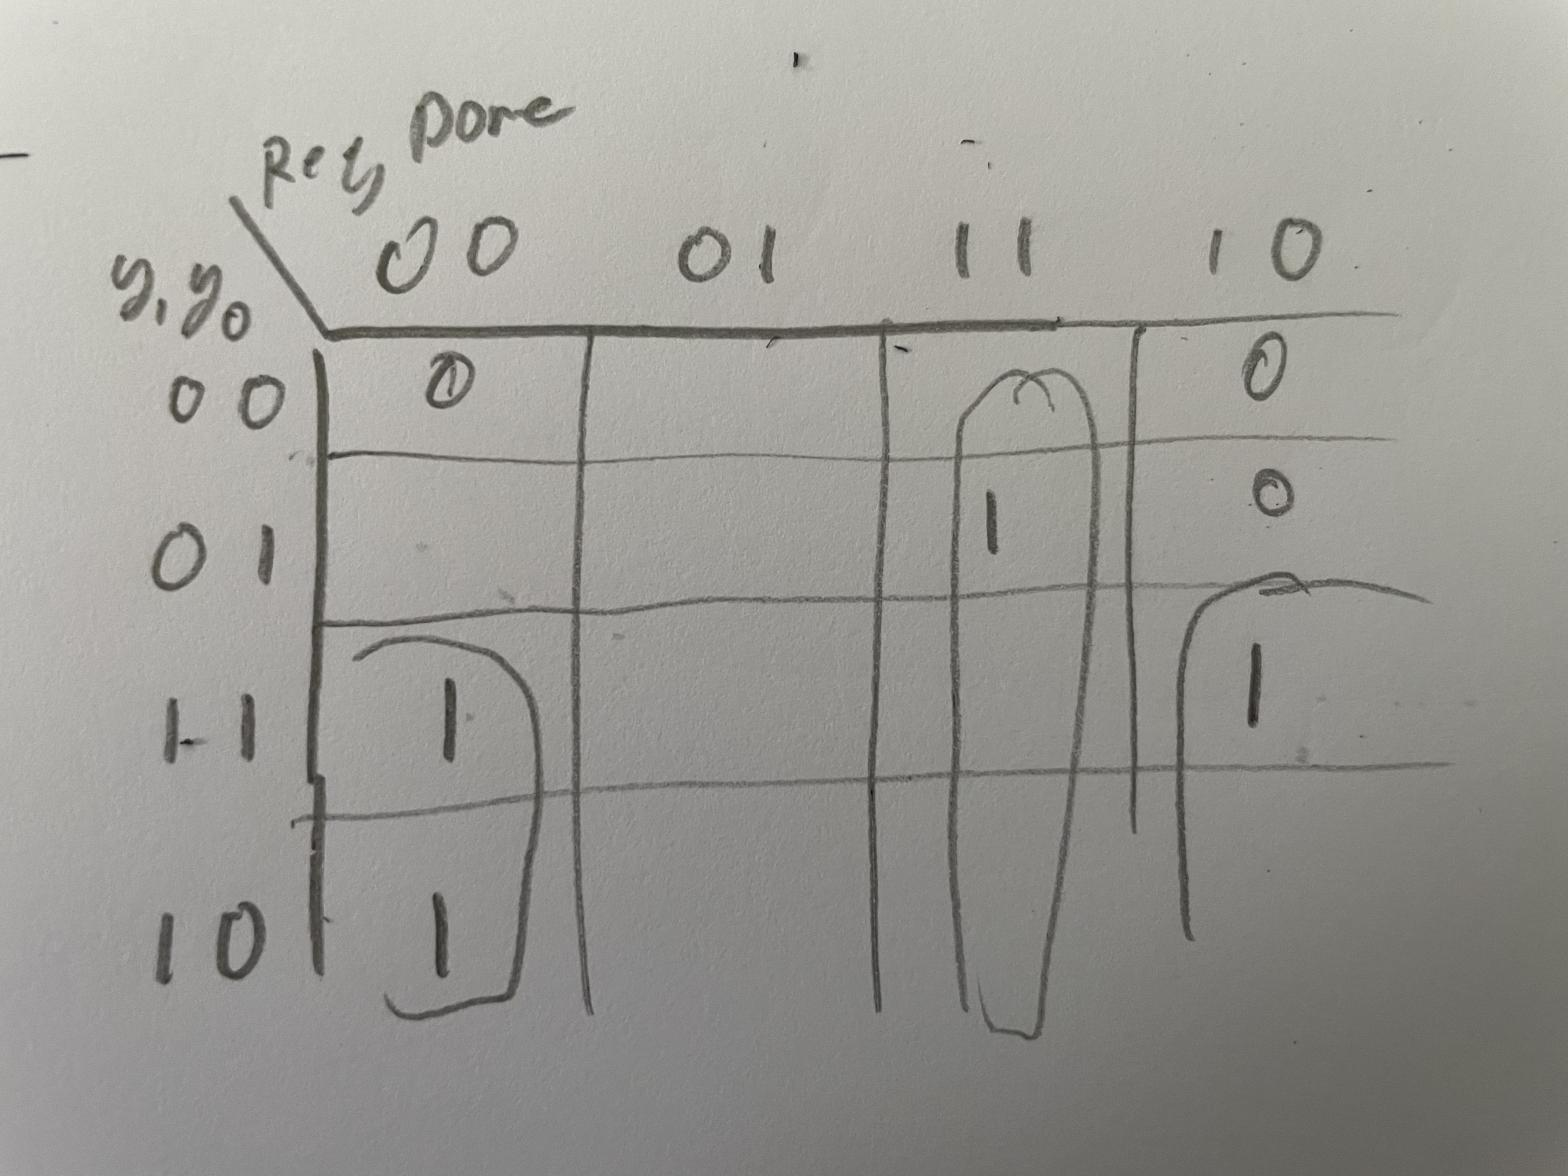
\includegraphics[scale=0.15]{fig20.jpg}\\
Which corresponds with the equation:
$$y_1^{n+1}=y_1^n.\overline{REQ}+DONE.REQ$$
Likewise the kmap for $y_0$ is shown below.\\
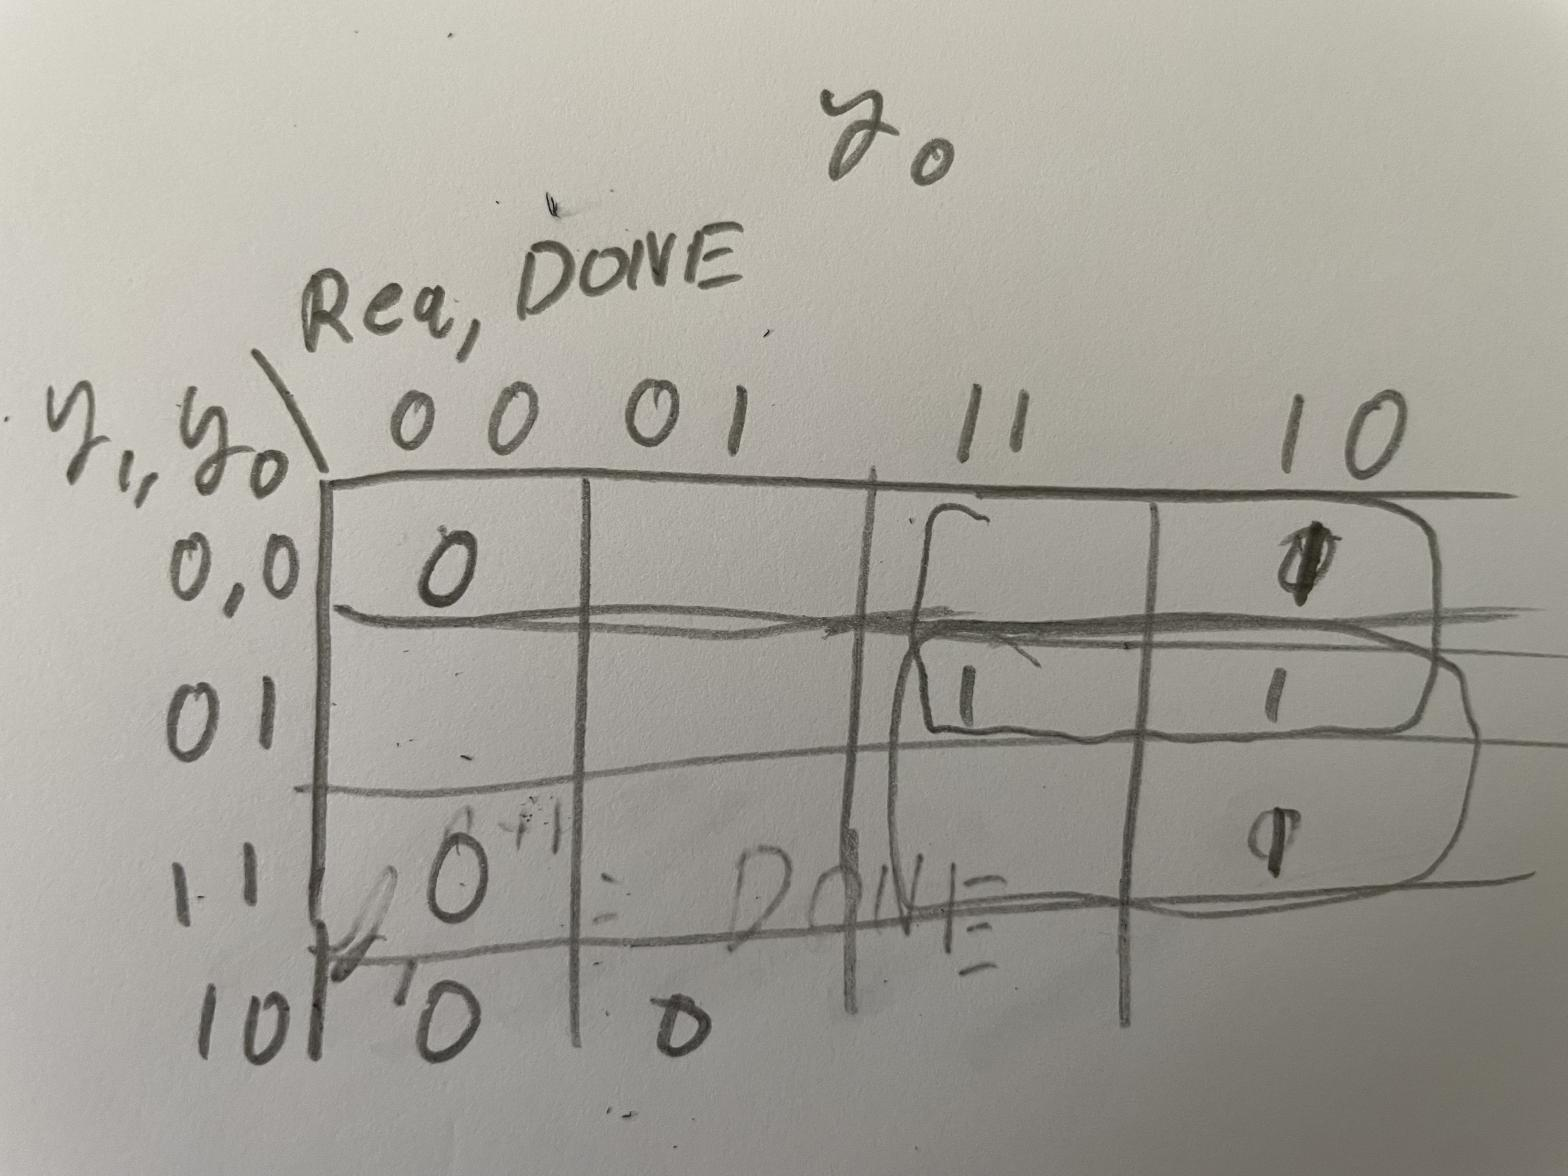
\includegraphics[scale=0.15]{fig21.jpg}\\
Which corresponds with the equation:
$$y_0^{n+1}=y_0^n.REQ+\overline{y_1^n}.REQ$$
We have that
\begin{align*}
    GO^{n+1}&=y_1^{n+1}.\overline{y_0^{n+1}}+\overline{y_1^{n+1}}.y_0^{n+1}\\
\end{align*}
And
\begin{align*}
    ACK^{n+1}&=y_1^{n+1}\\
    &=y_1^n.\overline{REQ}+DONE.REQ
\end{align*}


\section*{Problem 7}
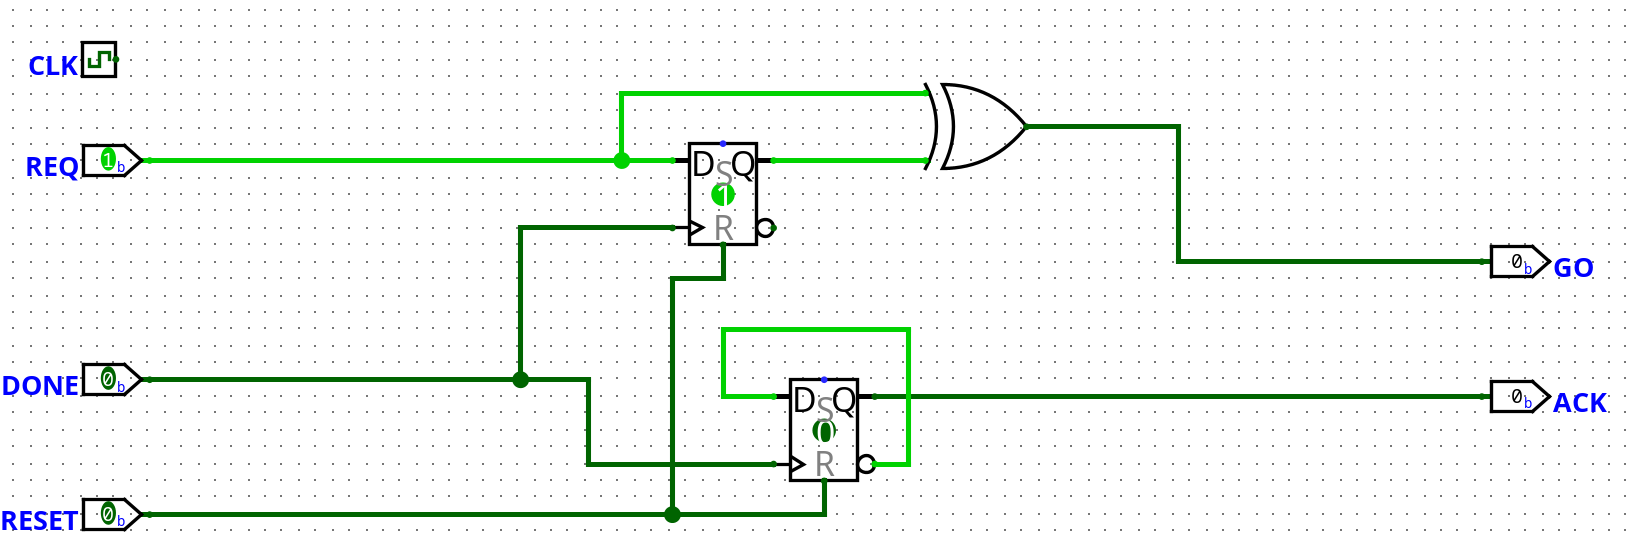
\includegraphics[scale=0.25]{fig14.png}\\
And has a chronograph of:\\
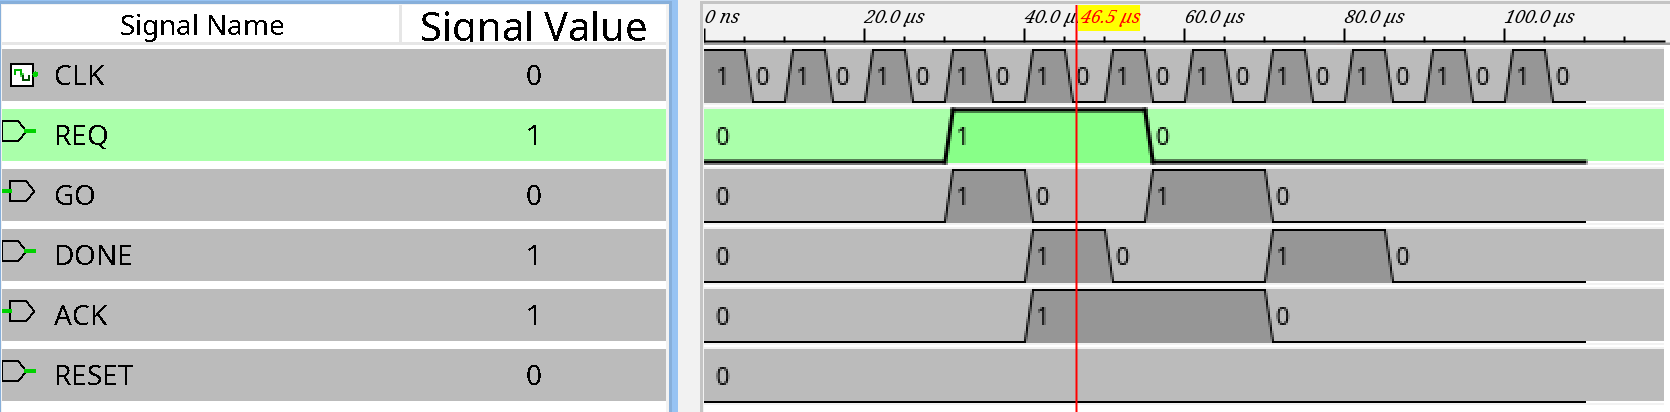
\includegraphics[scale=0.25]{fig15.png}
\section*{Problem 8}
Using the following flow chart\\
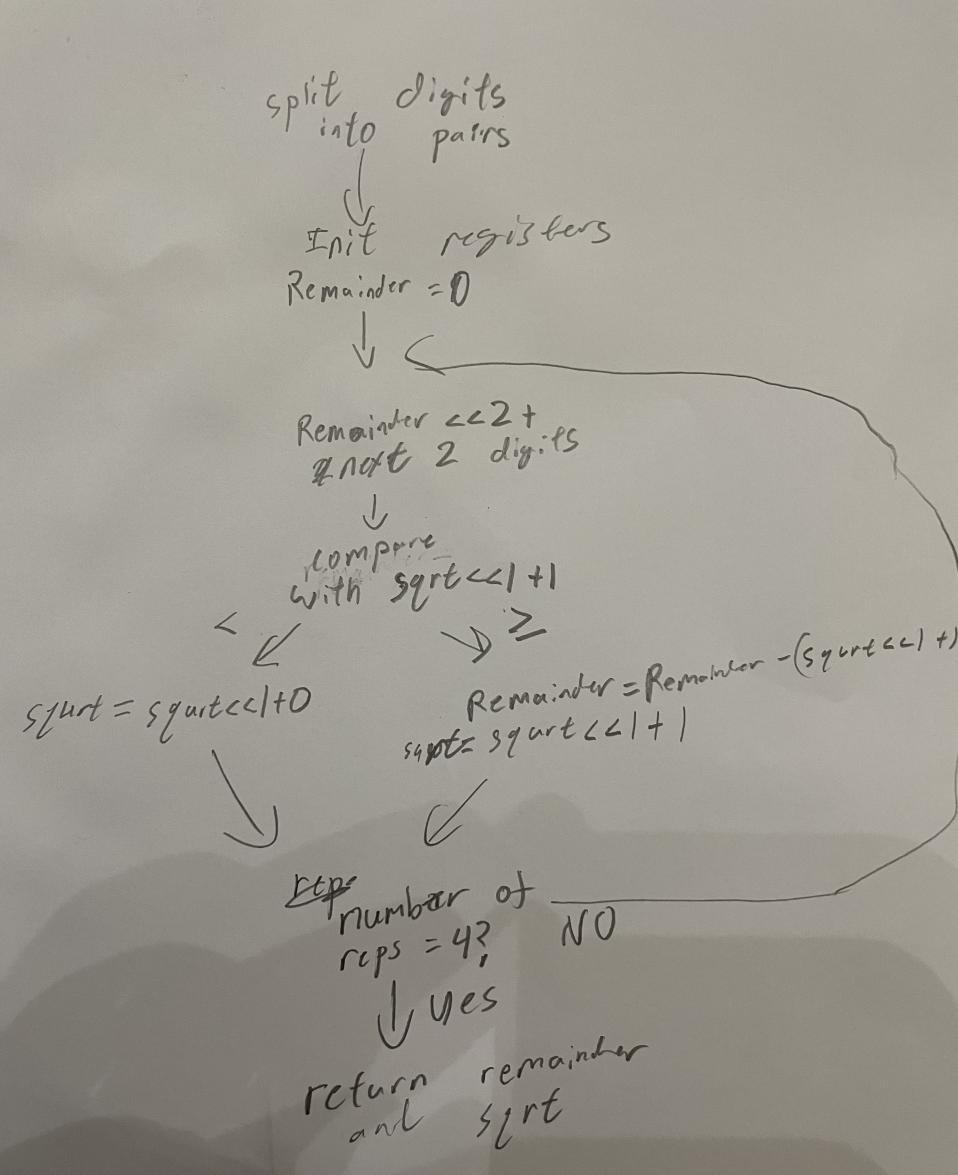
\includegraphics[scale=0.25]{fig9.jpg}\\
I created the circuit\\
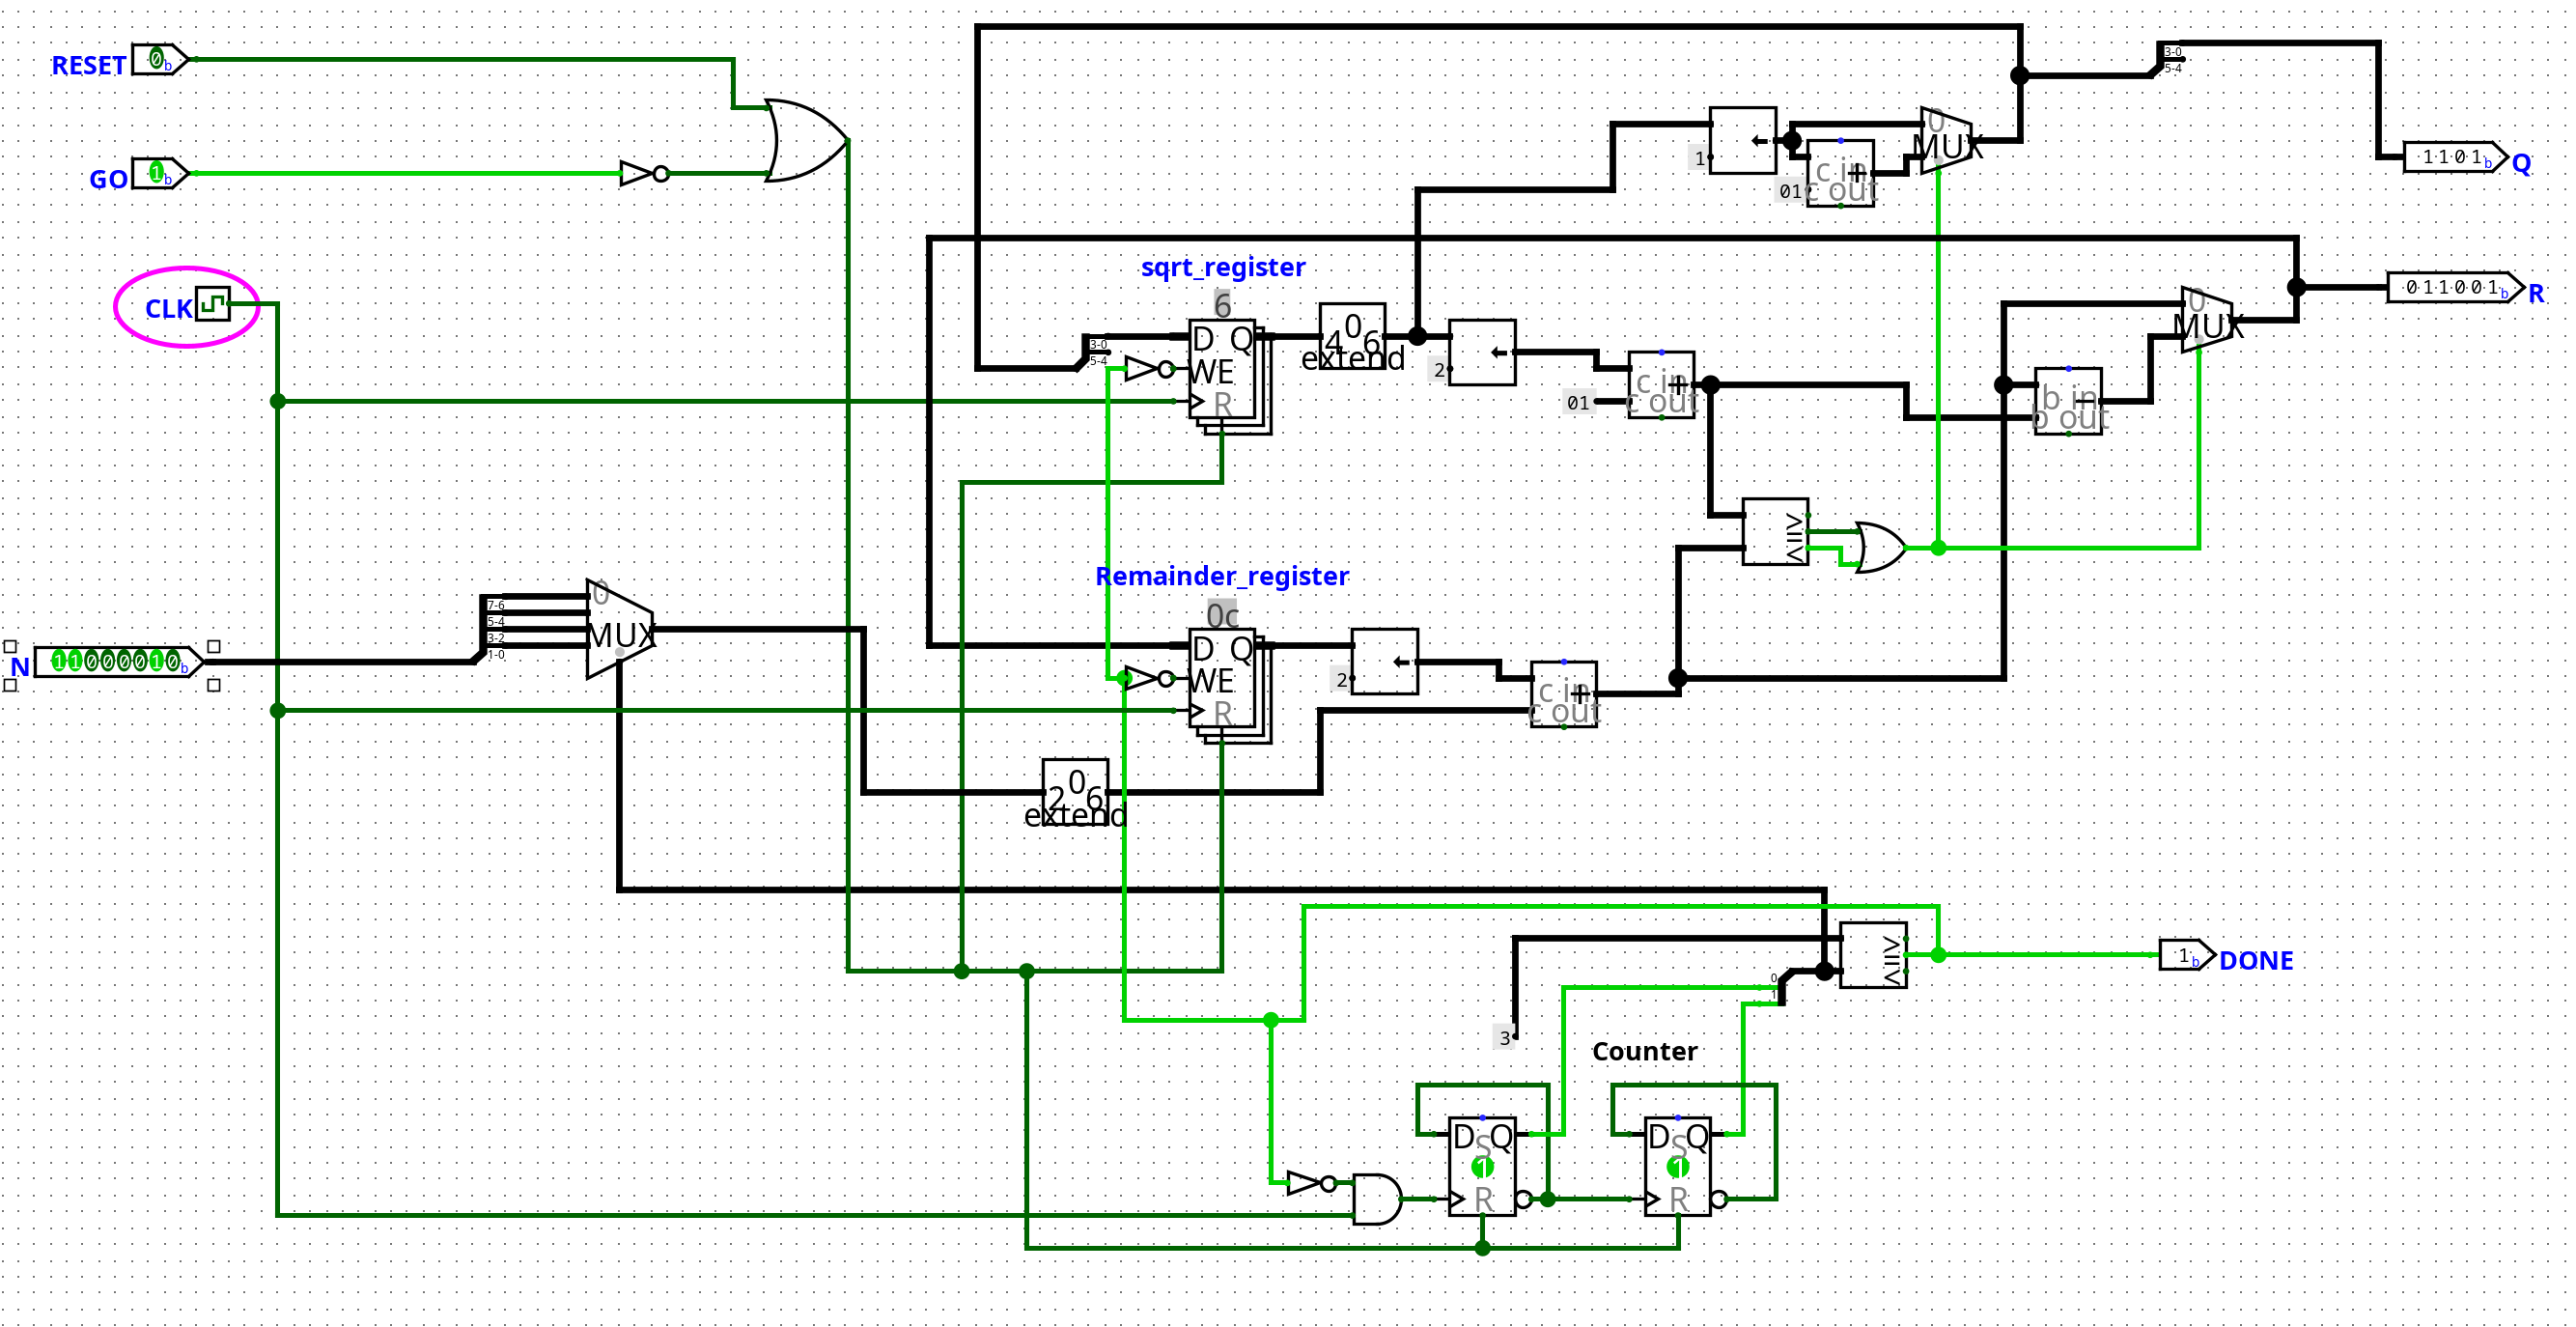
\includegraphics[scale=0.25]{fig10.png}
\end{document}
